\documentclass{article}
\renewcommand{\familydefault}{\sfdefault}

\usepackage{amssymb}
\usepackage{booktabs}
\usepackage{float}
\usepackage{geometry}
\usepackage{graphicx}
\usepackage{listings}
\usepackage{parskip}
\usepackage{xcolor}
\usepackage[colorlinks]{hyperref}
\usepackage[nameinlink,noabbrev]{cleveref} % Load after hyperref

\geometry{margin=2cm}

\definecolor{brick-red}{RGB}{203,65,84}

\lstset{
    backgroundcolor=\color[gray]{0.95},
    basicstyle=\ttfamily\footnotesize,
    commentstyle=\color{brick-red},
    frame=single,
    framerule=0pt,
    framextopmargin=1em,
    framexbottommargin=1em,
    framexleftmargin=1em,
    framexrightmargin=1em,
    keepspaces=true,
    numbers=none,
    showstringspaces=false,
    xrightmargin=2em,
    xleftmargin=2em,
}

\definecolor{cite-color}{RGB}{206,34,120}
\definecolor{link-color}{RGB}{28,172,184}
\definecolor{file-color}{RGB}{124,195,3}
\definecolor{url-color}{RGB}{102,35,175}

\AtBeginDocument{
	\hypersetup{
	    citecolor=link-color,
	    linkcolor=cite-color,
	    filecolor=file-color,
	    urlcolor=url-color
	}
 }

\title{Illumina vs. AVITI}

\author{thomas silvers}

\begin{document}

\maketitle

We performed two sequencing experiments on a library prepared from a pool of samples. In one experiment, Illumina sequencing was used; in the other, AVITI.
To compare results, we restrict our analysis to \textit{E. coli} samples from a single donor (Baby 2, \texttt{B002}).

\section{Number of reads}

We used \texttt{fastp} to trim, filter, and tally reads with pseudocode:

\begin{lstlisting}[language=bash]
$ fastp {input FASTQs} \ 
  --cut_front \
  --cut_tail \
  --trim_poly_x \
  --cut_mean_quality 30 \ 
  --qualified_quality_phred 30 \
  --unqualified_percent_limit 10 \
  --length_required 50
\end{lstlisting}
    
Results were collected using MultiQC and parsed using custom code.

\textbf{Results}

\begin{itemize}
    \item \textcolor{red}{AVITI} has $\sim 10^9$ reads, even after filtering (\cref{figure:reads})
\end{itemize}

\begin{figure}[H]
    \centering
    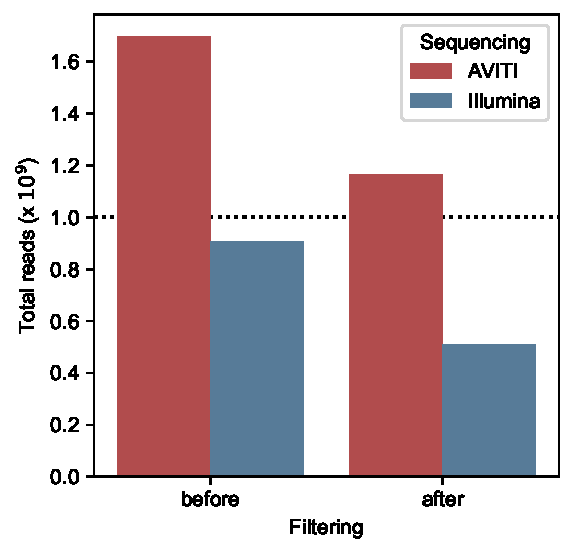
\includegraphics[width=.45\textwidth]{figures/total_reads.pdf}
    \caption{
        \textbf{Total number of reads} for \textcolor{red}{AVITI} or \textcolor{blue}{Illumina}, before and after filtering with \texttt{fastp}.
    }
    \label{figure:reads}
\end{figure}

\section{Variant quality scores}

We used \texttt{bcftools} to generate pile-ups and \texttt{bcftools stats} to extract variant quality scores with pseudocode:

\begin{lstlisting}[language=bash]
$ bcftools mpileup --fasta-ref {reference} --min-BQ 20 {bam} \
    | bcftools call --output-type v --ploidy 1 --multiallelic-caller \
    | bcftools reheader --samples sample_name.list \
    | bcftools view --output-file {prefix}.vcf.gz --output-type z
$ tabix -p vcf -f {prefix}.vcf.gz
$ bcftools stats {prefix}.vcf.gz > {prefix}.bcftools_stats.txt
\end{lstlisting}
    
Results were collected using MultiQC and parsed using custom code.

\textbf{Results}

\begin{itemize}
    \item \textcolor{red}{AVITI} has slightly higher, though comparable, variant quality scores compared with \textcolor{blue}{Illumina} (\cref{figure:variants})
\end{itemize}

\begin{figure}[H]
    \centering
    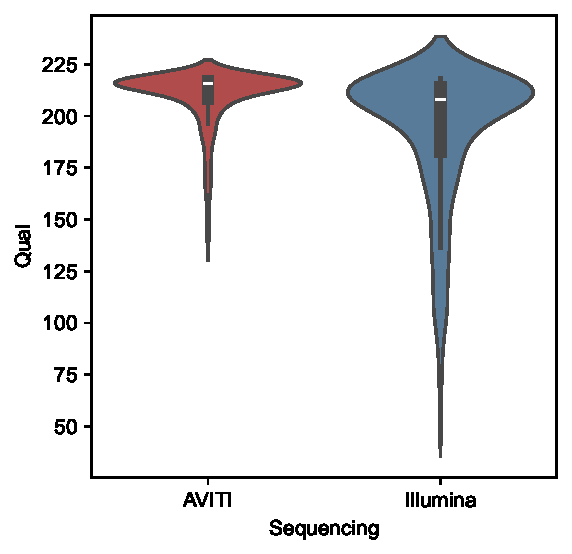
\includegraphics[width=.45\textwidth]{figures/variant_quality_scores.pdf}
    \caption{
        \textbf{Variant quality scores} for \textcolor{red}{AVITI} or \textcolor{blue}{Illumina}.
    }
    \label{figure:variants}
\end{figure}

\section{Sequence typing}

We used \texttt{srst2} to perform sequence typing for E. coli (MLST database name \texttt{Escherichia coli\#1}) with pseudocode:

\begin{lstlisting}[language=bash]
$ srst2 --input_pe {trimmed reads} --mlst_* '{Escherichia_coli#1}'
\end{lstlisting}

\textbf{Results}

\begin{itemize}
    \item $\frac{250}{256} \approx 98\%$ agreement between \textcolor{red}{AVITI} and \textcolor{blue}{Illumina} (\cref{tab:st})
    \item \textcolor{red}{AVITI} (\textcolor{red}{$\diamond$}) has higher seq. depth at core genes used for sequence typing than \textcolor{blue}{Illumina} (\textcolor{blue}{$\bullet$}) (\cref{figure:st})
    \item \texttt{(ST)73} is the dominant sequence type (\cref{figure:st})
\end{itemize}

\begin{figure}[H]
    \centering
    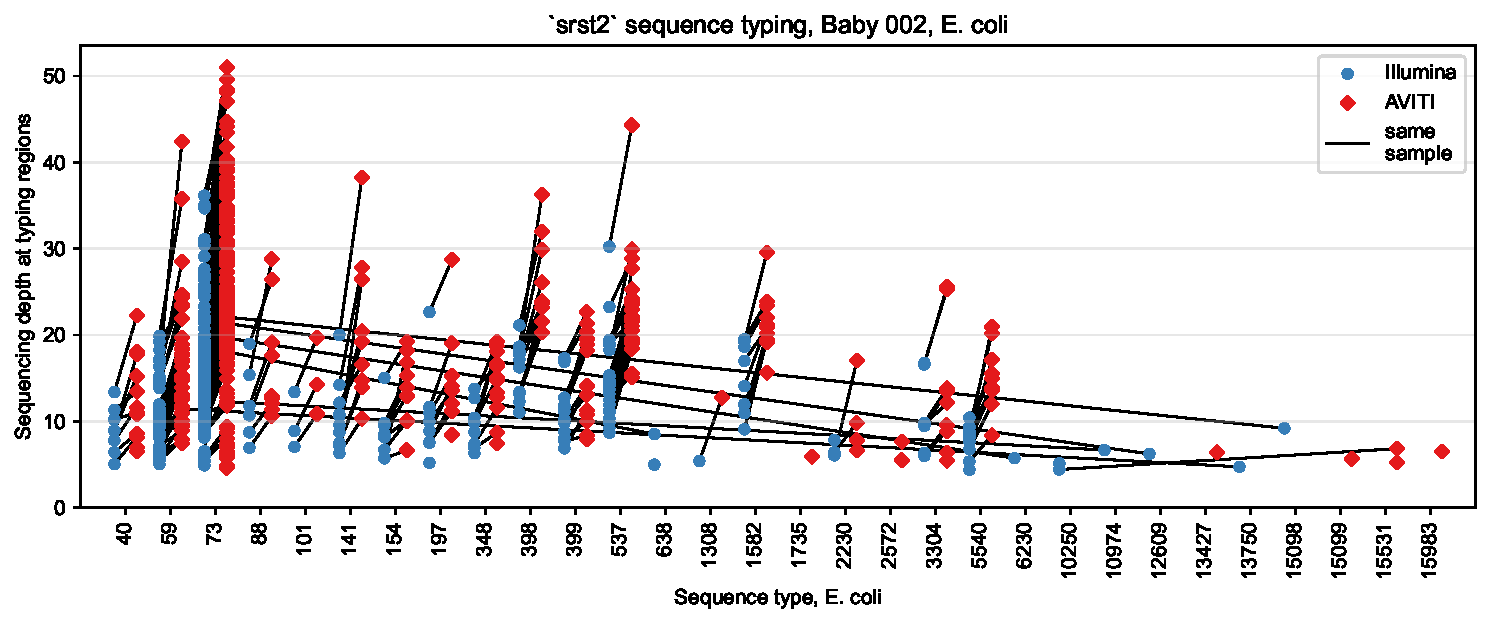
\includegraphics[width=.95\textwidth]{figures/sequence_typing.pdf}
    \caption{
        \textbf{Sequence typing results} for successful \texttt{srst2} sequence typing of identical samples ($-$) 
        prepared using \textcolor{red}{AVITI} (\textcolor{red}{$\diamond$}) or \textcolor{blue}{Illumina} (\textcolor{blue}{$\bullet$}).
    }
    \label{figure:st}
\end{figure}

\begin{table}[H]
    \centering
    \begin{tabular}{lr}
\toprule
 & Count \\
\midrule
AVITI \& Illumina (total) & 398 \\
AVITI, typed (total) & 379 \\
Illumina, typed (total) & 331 \\
AVITI \& Illumina, typed (total) & 312 \\
AVITI \& Illumina, typed (agree) & 305 \\
\bottomrule
\end{tabular}

    \caption{
        \textbf{Summary of sequence typing results}, tallying the number of samples for different criteria. 
        The top row provides the total number of samples; 
        the bottom row provides the number of samples \textit{successfully} sequence typed for \textit{both} AVITI \textit{and} Illumina 
        \textit{and agree} in the designated sequence type.
    }
    \label{tab:st}
\end{table}

\section{Reconstructing phylogenies of dominant STs}

We used \texttt{raxml-ng} to infer the phylogeny of samples from the dominant sequence type with pseudocode:

\begin{lstlisting}[language=bash]
$ raxml-ng --search1 --model GTR+G --outgroup {outgroup} --msa {msa}
\end{lstlisting}

We used $1000$ randomly sampled positions with an ALT allele called in at least 2 samples that met the following criteria:

\begin{itemize}
    \item No indels
    \item $\geq 3$ reads supporting ALT on each strand
    \item MAF $\geq .95$
    \item QUAL $\geq 30$
\end{itemize}

A final phylogeny would use full pseudogenomes and estimate bootstrap intervals. We find that a low depth cut-off is required, otherwise many \textcolor{blue}{Illumina} (\textcolor{blue}{$\bullet$}) 
calls are filtered out (\cref{figure:variant-call-disagree})

\begin{figure}[H]
    \centering
    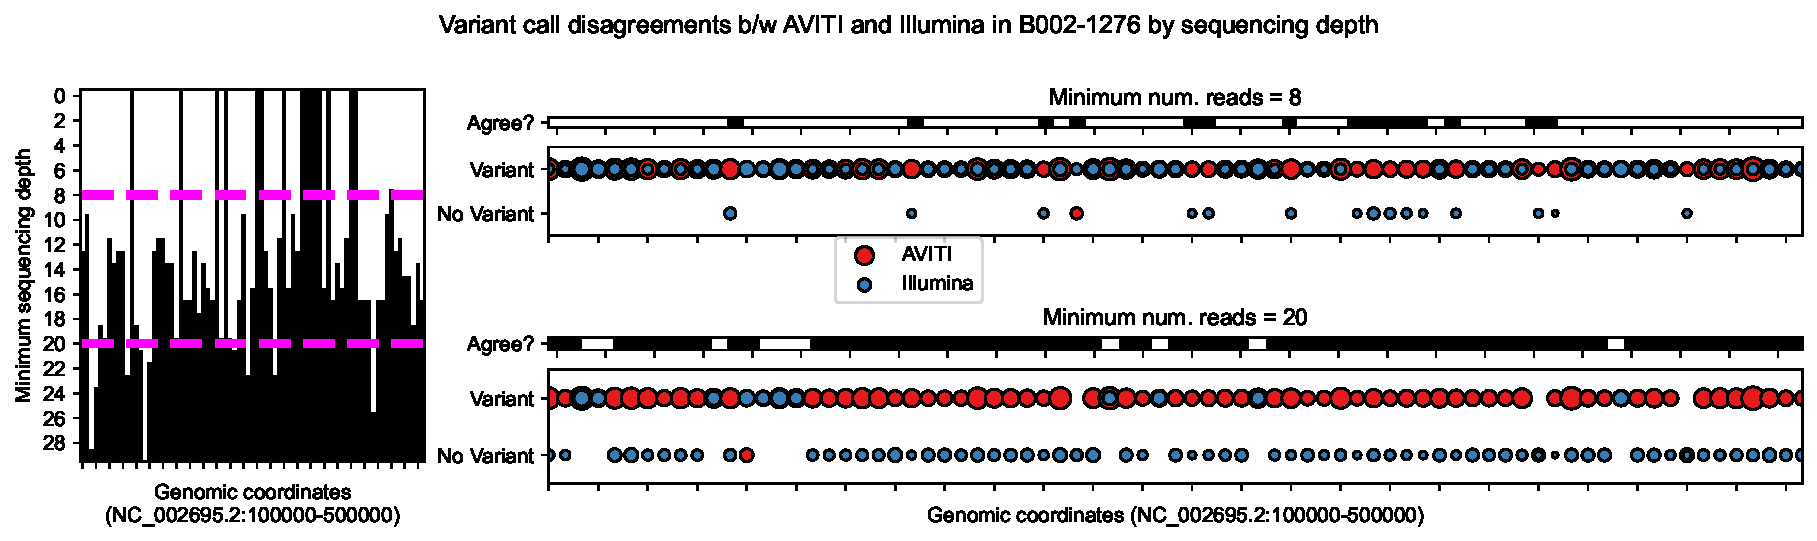
\includegraphics[width=.95\textwidth]{figures/variant-call-disagree}
    \caption{
        \textbf{Variant call disagreements} are mainly caused by combining the higher depth of AVITI and sequencing metrics thresholds. 
        A case study of sample \texttt{B002-1276} shows that \textcolor{red}{AVITI} (\textcolor{red}{$\bullet$}) and \textcolor{blue}{Illumina} (\textcolor{blue}{$\bullet$}) call nearly
        identical variants (agree $=\square$, disagree $=\blacksquare$) when the minimum required depth of a variant call (number of overlapping reads with the alt allele) is low (\textit{see left plot}).
        For instance, at the cut-off $=8$, there is agreement at all but 15 sites (\textit{top-right plots}). 
        Marker size is relative to sequencing depth; note the higher depth for \textcolor{red}{AVITI} (\textcolor{red}{$\bullet$}). 
        At a higher cut-off value ($20$), there are now numerous disagreements (\textit{left and bottom-right plots}).
    }
    \label{figure:variant-call-disagree}
\end{figure}

The two sample phylogenies, from \textcolor{red}{AVITI} and \textcolor{blue}{Illumina}, show agreement (Robinson-Foulds agreement metric between two trees $=0.658$; \cref{figure:tree-metrics-comp}). 
See a combined tree from a random subset of samples at \url{https://transfer.mpiib-berlin.mpg.de/f/14297709} (a more legible version with some samples highlighted is at \url{https://transfer.mpiib-berlin.mpg.de/f/14297708}).

\begin{figure}[H]
    \centering
    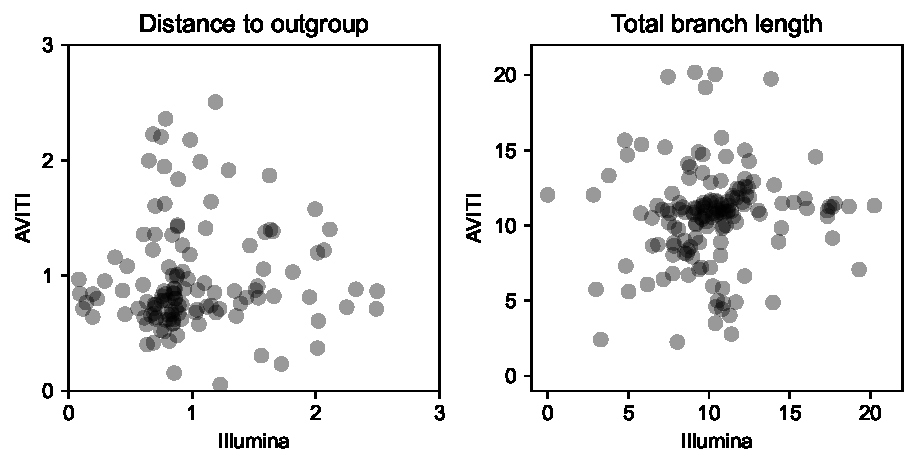
\includegraphics[width=.6\textwidth]{figures/tree-metrics-comp}
    \caption{
        \textbf{Comparing tree metrics} for AVITI and Illumina from trees built using \texttt{raxml-ng}.
    }
    \label{figure:tree-metrics-comp}
\end{figure}

\section{Appendix}

Code to reproduce is available on GitHub at \href{https://github.com/t-silvers/sequencing-comparison-aviti-illumina}{t-silvers/sequencing-comparison-aviti-illumina}.

\end{document}